\documentclass[hyperref={pdfpagelabels=false},usepdftitle=false]{beamer}
\usepackage{../templates/myStyle}

\begin{document}

\title{\titleText}
\subtitle{}
\author{\tutor}
\date{25. Februar 2014}
\subject{Proseminar Informatik}

\frame{\titlepage}

%\frame{
%    \frametitle{Inhalte}
%    \setcounter{tocdepth}{1}
%    \tableofcontents
%    \setcounter{tocdepth}{2}
%}

\section{Szenario}
\subsection{Zitationsdatenbanken}
\begin{frame}{Zitationsdatenbanken}
    \begin{itemize}
        \item \textbf{Publikationen} oder \textbf{Autoren} können \textbf{Knoten} sein,
        \item \textbf{Zitate} oder \textbf{Mehrautorenschaft}können \textbf{Kanten} sein und
        \item \textbf{Kategorien} können \textbf{Beschriftungen} sein
    \end{itemize}

    \textbf{Problem}: Nicht alle Knoten sind beschriftet

    \textbf{Anwendungsideen}:
    \begin{itemize}
        \item Kategorievorschläge bei neuen Einträgen
        \item Korrekturvorschläge für alte Einträge
    \end{itemize}
\end{frame}

\begin{frame}{}
    \textbf{Herausforderungen}
    \begin{itemize}
        \item Große Graphen,
        \item Dynamische Graphen,
        \item Texte sollen verwendet werden
    \end{itemize}

    \begin{table}
        \begin{tabular}{|l||r|r|r|r|}\hline
        \textbf{Name} & \textbf{Knoten} & \textbf{davon beschriftet} & \textbf{Kanten}  & \textbf{Beschriftungen} \\ \hline\hline
        \textbf{CORA} & \num{19396}  & \num{14814}             & \num{75021}   & 5              \\
        \textbf{DBLP} & \num{806635} & \num{18999 }            & \num{4414135} & 5              \\\hline
        \end{tabular}
    \end{table}

    \uncover<2>{
        \textbf{DYCOS} ist
        \begin{itemize}
            \item effizient,
            \item einfach,
            \item und nutzt Struktur und Texte
        \end{itemize}
    }
\end{frame}

\framedgraphic{Zitationsdatenbanken}{../images/literaturdatenbank.pdf}
\framedgraphic{Social Network}{../images/unlabeled-network}
\framedgraphic{Partially labeled network}{../images/partially-labeled-network}
\framedgraphic{Partially labeled network with content}{../images/partially-labeled-network-context.png}


\section{Überblick}
\subsection{Überblick}
\begin{frame}{Überblick}
    \begin{itemize}
        \item Graph ist gegeben
        \item Knoten sind teilweise beschriftet
        \item Fehlende Beschriftungen sollen berechnet werden
    \end{itemize}

    \uncover<2>{
    \textbf{Idee}: Homophilie nutzen\\
    Nahe Knoten sind ähnlich\\
    $\Rightarrow$ Random Walks zur Klassifizierung nutzen
    }
\end{frame}

\pgfdeclarelayer{background}
\pgfsetlayers{background,main}

\tikzstyle{vertex}=[circle,fill=black!25,minimum size=20pt,inner sep=0pt]
\tikzstyle{selected vertex} = [vertex, fill=red!24]
\tikzstyle{blue vertex} = [vertex, fill=blue!24]
\tikzstyle{edge} = [draw,thick,-]
\tikzstyle{weight} = [font=\small]
\tikzstyle{selected edge} = [draw,line width=5pt,-,red!50]
\tikzstyle{ignored edge} = [draw,line width=5pt,-,black!20]

\begin{frame}{Knotenklassifizierung mit Random Walks}
    \begin{figure}
        \begin{tikzpicture}[->,scale=1.8, auto,swap]
            % Draw the vertices. First you define a list.
            \foreach \pos/\name/\ltext in {{(0,0)/a/}, {(0,2)/b/b}, {(1,2)/c/},
                                    {(1,0)/d/}, {(2,1)/e/e}, {(3,1)/f/b},
                                    {(4,2)/g/a}, {(5,2)/h/a}, {(4,0)/i/a},
                                    {(5,0)/j/}}
                \node[draw,circle,fill=white] (\name) at \pos {$\ltext$};

            \node[draw,circle,red,fill=red] (e) at (2,1) {$e$};

            % Connect vertices with edges and draw weights
            \foreach \source/ \dest /\pos in {a/b/, b/c/, c/d/, d/a/,
                                        c/e/bend left, d/e/, e/c/,
                                        e/f/, f/g/, f/i/,
                                        g/f/bend right, i/f/bend left,
                                        g/h/, h/j/, j/i/, i/g/}
                \path (\source) edge [\pos] node {} (\dest);

            \foreach \fr / \number in {1/,
                2/b=1,
                3/b=1\, a=1,
                4/b=1\, a=2,
                5/b=2\, a=2,
                6/b=2\, a=3,
                7/b=2\, a=4,
                13/b=3\, a=4
                }
                \node<\fr->[fill=white] (Tlabel) at (2,0) {$\number$};

            % Start animating the edge selection.
            % For convenience we use a background layer to
            % highlight edges. This way we don't have to worry about
            % the highlighting covering weight labels.
            \begin{pgfonlayer}{background}
                \foreach \source / \dest / \fr / \colorf /\pos in {e/f/2/red/,f/g/3/red/,g/h/4/red/, e/f/5/blue/, f/i/6/blue/, i/g/7/blue/,e/c/8/green/,c/d/9/green/, d/a/10/green/,e/c/11/yellow/,c/e/12/yellow/bend left,e/f/13/yellow/}
                    \path<\fr->[selected edge, \colorf!20] (\source.center) edge
                                        [\pos] node {} (\dest.center);
            \end{pgfonlayer}
        \end{tikzpicture}
    \end{figure}

    Klassifizieren des roten Knotens:
    \begin{itemize}
        \item Zählen von Knotenbeschriftungen in Random Walks
        \item 4 Random Walks, beginnend bei Rot
        \item 3 Sprünge pro Random Walk
        \item<14> $4 \cdot a$, $3 \cdot b \Rightarrow$ Rot mit $a$ klassifizieren
    \end{itemize}
\end{frame}

\begin{frame}{Wortknoten}
    \begin{itemize}
        \item Bisher wurden keine Texte genutzt
        \item Idee: Graph erweitern
        \begin{itemize}
            \item Texte als Wortmengen
            \item Strukturknoten verweisen auf Wortknoten
            \item vice versa
        \end{itemize}
    \end{itemize}
\end{frame}

\framedgraphic{}{../images/wortknoten-visualisierung.pdf}
\framedgraphic{Erweiterter, semi-bipartiter Graph}{../images/graph-content-and-structure.pdf}


\section{Vokabular}
\subsection{Vokabular}
\begin{frame}{Vokabular}
    \begin{itemize}
        \item<1-> Füllwörter: und, oder, im, in, \dots
        \item[$\Rightarrow$]<2-> Beschränkung des Vokabulars sinnvoll
    \end{itemize}

    \uncover<3->{
    \textbf{Idee}:
    \begin{itemize}
        \item<4-> Zufällige Beispielmenge von Texten für Vokabularbildung betrachten
        \item<5-> Gini-Koeffizient nutzen
    \end{itemize}
    }
\end{frame}

\begin{frame}{Gini-Koeffizient}
    \begin{itemize}
        \item<1-> statistisches Maß für Ungleichverteilung
        \item<2-> $g = \sum_i p_i^2$ mit $p_i$ als relative Häufigkeit
        \item<3-> Hier: $g \in (0, 1]$
        \item<4-> $g$ nahe bei $1$ $\Rightarrow$ Wort ist stark ungleich verteilt
        \item[$\Rightarrow$]<5-> Nehme Top-$m$ Wörter mit höchstem
                  Gini-Koeffizient
    \end{itemize}
\end{frame}

\begin{frame}{Gini-Koeffizient}
    \begin{center}
        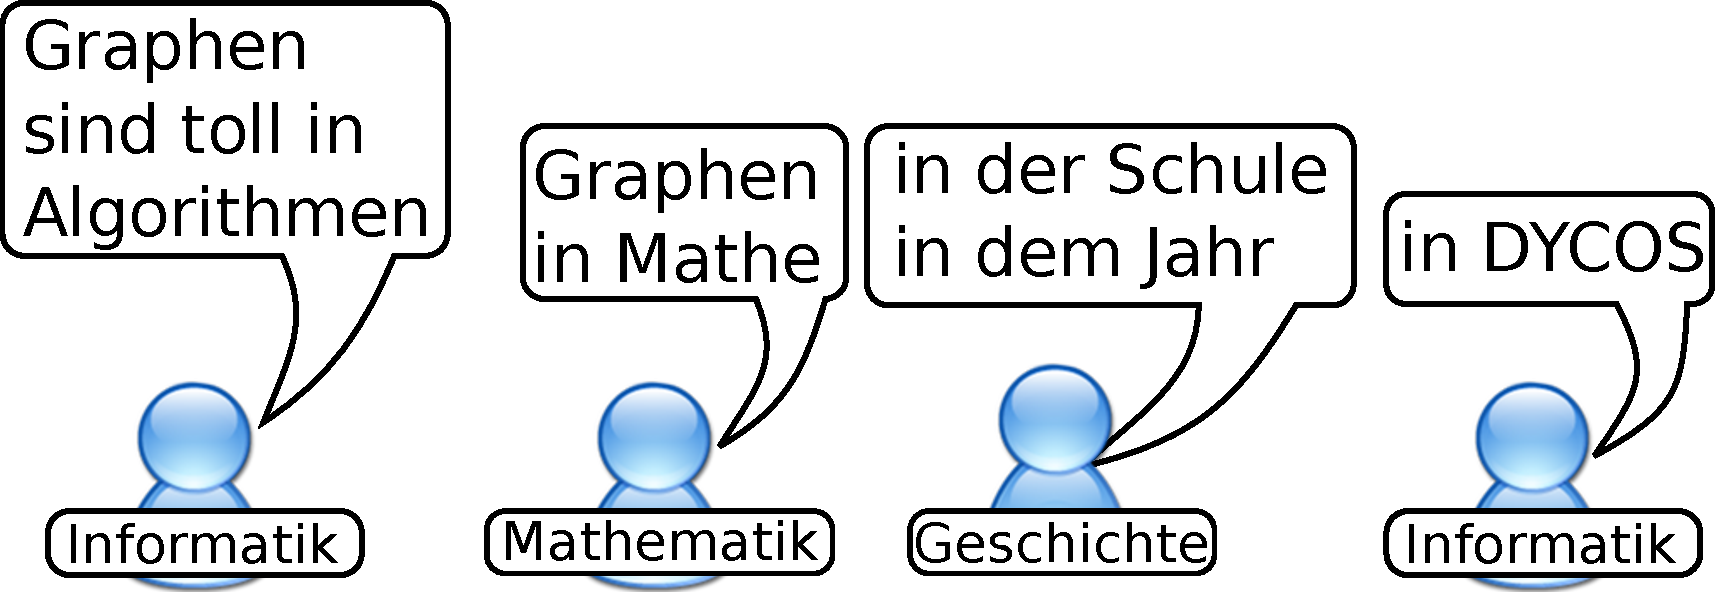
\includegraphics[width=\textwidth,height=0.4\textheight,keepaspectratio]{../images/gini-example.pdf}
    \end{center}

    \uncover<2->{Beispiel: \enquote{in}}
    \begin{itemize}
        \item<3-> Vorkommen insgesamt: $5 \times$
        \item<4-> Vorkommen in \enquote{Informatik} $2\times \Rightarrow p_1 = \frac{2}{5}$
        \item<5-> Vorkommen in \enquote{Mathematik} $1\times \Rightarrow p_2 = \frac{1}{5}$
        \item<6-> Vorkommen in \enquote{Geschichte} $2\times \Rightarrow p_3 = \frac{2}{5}$
        \item<7-> Gini-Koeffizient: $\left (\frac{2}{5} \right )^2 + \left (\frac{1}{5} \right )^2 + \left (\frac{2}{5} \right )^2 = \frac{9}{25}$
    \end{itemize}
\end{frame}


\section{Sprungtypen}
\subsection{Sprungtypen}\label{sec:sprungtypen}
Die beiden bereits definierten Sprungtypen, der strukturelle Sprung sowie der
inhaltliche Zweifachsprung werden im Folgenden erklärt.
\goodbreak
Der strukturelle Sprung entspricht einer zufälligen Wahl eines Nachbarknotens,
wie es in \cref{alg:DYCOS-structural-hop} gezeigt wird.
\begin{algorithm}[H]
    \begin{algorithmic}[1]
        \Procedure{SturkturellerSprung}{Knoten $v$, Anzahl $q$}
            \State $n \gets v.\Call{NeighborCount}{}$ \Comment{Wähle aus der Liste der Nachbarknoten}
            \State $r \gets \Call{RandomInt}{0, n-1}$ \Comment{einen zufällig aus}
            \State $v \gets v.\Call{Next}{r}$ \Comment{Gehe zu diesem Knoten}
            \State \Return $v$
        \EndProcedure
    \end{algorithmic}
\caption{Struktureller Sprung}
\label{alg:DYCOS-structural-hop}
\end{algorithm}

Bei inhaltlichen Zweifachsprüngen ist jedoch nicht sinnvoll so strikt nach der
Definition vorzugehen,  also direkt von einem strukturellem Knoten $v \in V_t$
zu einem mit $v$ verbundenen Wortknoten $w \in W_t$ zu springen und von diesem
wieder zu einem verbundenem strukturellem Knoten $v' \in V_t$. Würde dies
gemacht werden, wäre zu befürchten, dass aufgrund von Homonymen die Qualität der
Klassifizierung verringert wird. So hat \enquote{Brücke} im Deutschen viele
Bedeutungen. Gemeint sein können z.~B. das Bauwerk, das Entwurfsmuster der
objektorientierten Programmierung oder ein Teil des Gehirns.

Deshalb wird für jeden Knoten $v$, von dem aus ein inhaltlicher
Zweifachsprung gemacht werden soll folgende Textanalyse durchgeführt:
\begin{enumerate}[label=C\arabic*,ref=C\arabic*]
    \item \label{step:c1} Gehe alle in $v$ startenden Random Walks der Länge $2$ durch
          und erstelle eine Liste $L$ der erreichbaren Knoten $v'$. Speichere
          außerdem, durch wie viele Pfade diese Knoten $v'$ jeweils erreichbar
          sind.
    \item \label{step:c2} Betrachte im Folgenden nur die Top-$q$ Knoten bzgl.
          der Anzahl der Pfade von $v$ nach $v'$, wobei $q \in \mathbb{N}$
          eine zu wählende Konstante des DYCOS-Algorithmus ist.\footnote{Sowohl für den DBLP, als auch für den
CORA-Datensatz wurde in \cite[S. 364]{aggarwal2011} $q=10$ gewählt.}
          Diese Knotenmenge heiße im Folgenden $T(v)$ und $p(v, v')$ sei die
          Anzahl der Pfade von $v$ über einen Wortknoten nach $v'$.
    \item \label{step:c3} Wähle mit Wahrscheinlichkeit
          $\frac{p(v, v')}{\sum_{w \in T(v)} p(v, w)}$ den Knoten $v' \in T(v)$
          als Ziel des Zweifachsprungs.
\end{enumerate}

Konkret könnte also ein inhaltlicher Zweifachsprung sowie wie in
\cref{alg:DYCOS-content-multihop} beschrieben umgesetzt werden.
Der Algorithmus bekommt einen Startknoten $v \in V_T$ und
einen $q \in \mathbb{N}$ als Parameter. $q$ ist ein Parameter der
für den DYCOS-Algorithmus zu wählen ist. Dieser Parameter beschränkt
die Anzahl der möglichen Zielknoten $v' \in V_T$ auf diejenigen
$q$ Knoten, die $v$ bzgl. der Textanalyse am ähnlichsten sind.

In \cref{alg:l2} bis \cref{alg:l5} wird \cref{step:c1} durchgeführt und alle
erreichbaren Knoten in $reachableNodes$ mit der Anzahl der Pfade, durch die sie
erreicht werden können, gespeichert.

In \cref{alg:l6} wird \cref{step:c2} durchgeführt. Ab hier gilt
\[ |T| = \begin{cases}q               &\text{falls } |reachableNodes|\geq q\\
                     |reachableNodes| &\text{sonst }\end{cases}\]

Bei der Wahl der Datenstruktur von $T$ ist zu beachten, dass man in
\cref{alg:21} über Indizes auf Elemente aus $T$ zugreifen können muss.

In \cref{alg:l8} bis \ref{alg:l13} wird ein assoziatives Array erstellt, das
von $v' \in T(v)$ auf die relative Häufigkeit bzgl. aller Pfade von $v$ zu
Knoten aus den Top-$q$ abbildet.

In allen folgenden Zeilen wird \cref{step:c3} durchgeführt. In \cref{alg:15}
bis \cref{alg:22} wird ein Knoten $v' \in T(v)$ mit einer Wahrscheinlichkeit,
die seiner relativen Häufigkeit am Anteil der Pfaden der Länge 2 von $v$ nach
$v'$ über einen beliebigen Wortknoten entspricht ausgewählt und schließlich
zurückgegeben.

\begin{algorithm}
  \caption{Inhaltlicher Zweifachsprung}
  \label{alg:DYCOS-content-multihop}
    \begin{algorithmic}[1]
        \Procedure{InhaltlicherZweifachsprung}{Knoten $v \in V_T$, $q \in \mathbb{N}$}
            \State $erreichbareKnoten \gets$ leeres assoziatives Array\label{alg:l2}
            \ForAll{Wortknoten $w$ in $v.\Call{getWordNodes}{ }$}
                \ForAll{Strukturknoten $x$ in $w.\Call{getStructuralNodes}{ }$}
                    \If{$!erreichbareKnoten.\Call{hasKey}{x}$}
                        \State $erreichbareKnoten[x] \gets 0$
                    \EndIf
                    \State $erreichbareKnoten[x] \gets erreichbareKnoten[x] + 1$
                \EndFor
            \EndFor\label{alg:l5}
            \State \label{alg:l6} $T \gets \Call{max}{erreichbareKnoten, q}$
            \\
            \State \label{alg:l8} $s \gets 0$
            \ForAll{Knoten $x \in T$}
                \State $s \gets s + erreichbareKnoten[x]$
            \EndFor
            \State $relativeHaeufigkeit \gets $ leeres assoziatives Array
            \ForAll{Knoten $x \in T$}
                \State $relativeHaeufigkeit \gets \frac{erreichbareKnoten[x]}{s}$
            \EndFor\label{alg:l13}
            \\
            \State \label{alg:15} $random \gets \Call{random}{0, 1}$
            \State $r \gets 0.0$
            \State $i \gets 0$
            \While{$s < random$}
                \State $r \gets r + relativeHaeufigkeit[i]$
                \State $i \gets i + 1$
            \EndWhile

            \State $v \gets T[i-1]$ \label{alg:21}
            \State \Return $v$ \label{alg:22}
        \EndProcedure
    \end{algorithmic}
\end{algorithm}


\section{Evaluation}
\subsection{Experimentelle Evaluation}
\begin{frame}{Evaluation}
    \begin{table}
        \begin{tabular}{|l||r|r|r|r|}\hline
        \textbf{Name} & \textbf{Knoten} & \textbf{davon beschriftet} & \textbf{Kanten}  & \textbf{Beschriftungen} \\ \hline\hline
        \textbf{CORA} & \num{19396}  & \num{14814}             & \num{75021}   & 5              \\
        \textbf{DBLP} & \num{806635} & \num{18999 }            & \num{4414135} & 5              \\\hline
        \end{tabular}
    \end{table}
\end{frame}

\begin{frame}{Evaluation}
    \begin{itemize}
        \item<1-> Performance:
            \begin{itemize}
                \item<2-> Klassifizierung aller Knoten
                \item<3-> Intel Xeon $\SI{2.5}{\GHz}$ mit $\SI{32}{\giga\byte}$ RAM, $1$ Kern
                \item<4-> DBLP: $< \SI{25}{\second}$
                \item<5-> CORA: $< \SI{5}{\second}$
            \end{itemize}
        \item<6-> Klassifikationsgüte:
            \begin{itemize}
                \item<7-> CORA: 82\% - 84\%
                \item<8-> DBLP: 61\% - 66\%
            \end{itemize}
    \end{itemize}
\end{frame}


\section{Zusammenfassung}
\subsection{Zusammenfassung}
\begin{frame}{Wichtige Ideen}
    \begin{itemize}
        \item<1-> Random Walk
        \item<2-> Gini-Koeffizient
        \item<3-> Inhaltlicher Zweifachsprung
    \end{itemize}
\end{frame}

\begin{frame}{Was ist an DYCOS dynamisch?}
    \begin{itemize}
        \item<1-> DYCOS ist nur von der lokalen Situation abhängig
        \item<2-> Klassifizierung von einzelnen Knoten möglich
        \item<3-> Klassifizierung ist einfach
        \item<4->[$\Rightarrow$] Der Graph darf dynamisch sein; DYCOS funktioniert dennoch
    \end{itemize}
\end{frame}


\section{Ende}
\subsection{Aufgabe 3}
\begin{frame}{Aufgabe 3}
Zeigen Sie: Wenn der Graph eines Kreises bipartit ist, dann hat der Kreis gerade Länge.
\end{frame}

\pgfdeclarelayer{background}
\pgfsetlayers{background,main}
\begin{frame}{Aufgabe 3 - Lösung}
Idee: Knoten abwechselnd färben

    \tikzstyle{selected edge} = [draw,line width=5pt,-,black!50]
    \begin{center}
    \adjustbox{max size={\textwidth}{0.8\textheight}}{
    \begin{tikzpicture}
        \node[vertex] (a) at (0,0) {};
        \node[vertex] (b) at (2,0) {};
        \node[vertex] (c) at (2,2) {};
        \node[vertex] (d) at (0,2) {};
        \node[vertex] (e) at (1,4) {};

        \draw (a) -- (b) -- (c) -- (e) -- (d) -- (a);

        \node<2->[vertex, red] (a) at (0,0) {};
        \node<3->[vertex, blue] (b) at (2,0) {};
        \node<4->[vertex, red] (c) at (2,2) {};
        \node<5->[vertex, blue] (e) at (1,4) {};
        \node<6->[vertex, red] (d) at (0,2) {};

        \begin{pgfonlayer}{background}
            \path<3->[selected edge] (a.center) edge node {} (b.center);
            \path<4->[selected edge] (b.center) edge node {} (c.center);
            \path<5->[selected edge] (c.center) edge node {} (e.center);
            \path<6->[selected edge] (e.center) edge node {} (d.center);
            \path<7->[selected edge,lime] (d.center) edge node {} (a.center);
        \end{pgfonlayer}
    \end{tikzpicture}
    }
    \end{center}
\end{frame}

\subsection{Aufgabe 4}
\begin{frame}{Aufgabe 4}
Zeigen Sie: Ein Graph $G$ ist genau dann bipartit, wenn er nur Kreise
gerade Länge hat.
\end{frame}

\begin{frame}{Aufgabe 4: Lösung, Teil 1}
\underline{Vor.:} Sei $G = (E, K)$ ein zus. Graph. \pause

\underline{Beh.:} $G$ ist bipartit $\Rightarrow G$ hat keine Kreis ungerader Länge \pause

\underline{Bew.:} durch Widerspruch \pause

\underline{Annahme:} $G$ hat Kreis ungerader Länge \pause

$\xRightarrow[]{A.4}$ Ein Subgraph von $G$ ist nicht bipartit \pause

$\Rightarrow$ Widerspruch zu \enquote{$G$ ist bipartit} \pause

$\Rightarrow$ $G$ hat keinen Kreis ungerader Länge $\blacksquare$
\end{frame}

\begin{frame}{Aufgabe 4: Lösung, Teil 2}
\underline{Vor.:} Sei $G = (E, K)$ ein zus. Graph. \pause

\underline{Beh.:} $G$ hat keinen Kreis ungerader Länge $\Rightarrow G$ ist bipartit \pause

\underline{Bew.:} Konstruktiv \pause

Färbe Graphen mit Breitensuche $\blacksquare$
\end{frame}

\pgfdeclarelayer{background}
\pgfsetlayers{background,main}
\begin{frame}{Aufgabe 4 - Beispiel}
    \tikzstyle{selected edge} = [draw,line width=5pt,-,black!50]
    \begin{center}
    \adjustbox{max size={\textwidth}{0.8\textheight}}{
    \begin{tikzpicture}
        \node[vertex] (a) at (1,1) {};
        \node[vertex] (b) at (2,0) {};
        \node[vertex] (c) at (4,0) {};
        \node[vertex] (d) at (1,2) {};
        \node[vertex] (e) at (2,2) {};
        \node[vertex] (f) at (3,2) {};
        \node[vertex] (g) at (2,4) {};
        \node[vertex] (h) at (3,3) {};
        \node[vertex] (i) at (4,2) {};
        \node[vertex] (j) at (1,3) {};

        \draw (a) -- (b);
        \draw (a) -- (d);
        \draw (b) -- (e);
        \draw (b) -- (c);
        \draw (c) -- (f);
        \draw (d) -- (e);
        \draw (d) -- (j);
        \draw (e) -- (f);
        \draw (f) -- (i);
        \draw (g) -- (j);
        \draw (g) -- (h);

        \node<2->[vertex, red]  (a) at (1,1) {};
        \node<3->[vertex, blue] (b) at (2,0) {};
        \node<3->[vertex, blue] (d) at (1,2) {};
        \node<4->[vertex, red]  (c) at (4,0) {};
        \node<4->[vertex, red]  (e) at (2,2) {};
        \node<4->[vertex, red]  (j) at (1,3) {};
        \node<5->[vertex, blue] (f) at (3,2) {};
        \node<5->[vertex, blue] (g) at (2,4) {};
        \node<6->[vertex, red]  (h) at (3,3) {};
        \node<6->[vertex, red]  (i) at (4,2) {};

        \begin{pgfonlayer}{background}
            \path<3->[selected edge] (a.center) edge node {} (b.center);
            \path<3->[selected edge] (a.center) edge node {} (d.center);
            \path<4->[selected edge] (b.center) edge node {} (c.center);
            \path<4->[selected edge] (b.center) edge node {} (e.center);
            \path<4->[selected edge] (d.center) edge node {} (j.center);
            \path<4->[selected edge] (d.center) edge node {} (e.center);
            \path<5->[selected edge] (j.center) edge node {} (g.center);
            \path<5->[selected edge] (e.center) edge node {} (f.center);
            \path<5->[selected edge] (c.center) edge node {} (f.center);
            \path<6->[selected edge] (g.center) edge node {} (h.center);
            \path<6->[selected edge] (f.center) edge node {} (i.center);
        \end{pgfonlayer}
    \end{tikzpicture}
    }
    \end{center}
\end{frame}

\subsection{Aufgabe 9}
\begin{frame}{Aufgabe 9, Teil 1}
Im folgenden sind die ersten drei Graphen $G_1, G_2, G_3$ einer
Folge $(G_n)$ aus Graphen abgebildet. Wie sieht $G_4$ aus?

\begin{gallery}
    \galleryimage{graphs/triangular-1}
    \galleryimage{graphs/triangular-2}
    \galleryimage{graphs/triangular-3}
\end{gallery}
\end{frame}

\begin{frame}{Aufgabe 9, Teil 1 (Lösung)}
    \begin{center}
        \documentclass[varwidth=true, border=2pt]{standalone}
\usepackage{ifthen}
\usepackage{tikz}
\usetikzlibrary{calc}

\begin{document}
\tikzstyle{vertex}=[draw,red,fill=red,circle,
minimum size=10pt,inner sep=0pt]
\tikzstyle{edge}=[red, very thick]
\begin{tikzpicture}
    \newcommand{\n}{4}
    \foreach \y in {0, ..., \n}{
        \pgfmathsetmacro{\loopend}{{2*\n-\y}}
        \pgfmathsetmacro{\second}{{\y+2}}
        \foreach \x in {\y, \second,..., \loopend}{
            \ifthenelse{\n=\y}{\breakforeach}{}
            \node (n-\x\y)[vertex] at (\x,\y) {};

            \ifthenelse{\y=0}{}{\draw[edge] (\x,\y) -- (\x+1,\y-1);}
            \pgfmathtruncatemacro\X{\x}
            \ifthenelse{\X<\loopend}{\draw[edge] (\x,\y) -- (\x+2,\y);}{}
            \ifthenelse{\X=\loopend}{}{\draw[edge] (\x,\y) -- (\x+1,\y+1);}

        }
    }
\end{tikzpicture}
\end{document}

    \end{center}
\end{frame}

\begin{frame}{Aufgabe 9, Teil 1 (Lösung)}
    \begin{center}
        \documentclass[varwidth=true, border=2pt]{standalone}
\usepackage{ifthen}
\usepackage{tikz}
\usetikzlibrary{calc}

\begin{document}
\tikzstyle{vertex}=[draw,red,fill=red,circle,
minimum size=10pt,inner sep=0pt]
\tikzstyle{edge}=[red, very thick]
\begin{tikzpicture}
    \newcommand{\n}{5}
    \foreach \y in {0, ..., \n}{
        \pgfmathsetmacro{\loopend}{{2*\n-\y}}
        \pgfmathsetmacro{\second}{{\y+2}}
        \foreach \x in {\y, \second,..., \loopend}{
            \ifthenelse{\n=\y}{\breakforeach}{}
            \node (n-\x\y)[vertex] at (\x,\y) {};

            \ifthenelse{\y=0}{}{\draw[edge] (\x,\y) -- (\x+1,\y-1);}
            \pgfmathtruncatemacro\X{\x}
            \ifthenelse{\X<\loopend}{\draw[edge] (\x,\y) -- (\x+2,\y);}{}
            \ifthenelse{\X=\loopend}{}{\draw[edge] (\x,\y) -- (\x+1,\y+1);}

        }
    }
\end{tikzpicture}
\end{document}

    \end{center}
\end{frame}

\begin{frame}{Aufgabe 9, Teil 1 (Lösung)}
    \begin{center}
        \documentclass[varwidth=true, border=2pt]{standalone}
\usepackage{ifthen}
\usepackage{tikz}
\usetikzlibrary{calc}

\begin{document}
\tikzstyle{vertex}=[draw,red,fill=red,circle,
minimum size=10pt,inner sep=0pt]
\tikzstyle{edge}=[red, very thick]
\begin{tikzpicture}
    \newcommand{\n}{6}
    \foreach \y in {0, ..., \n}{
        \pgfmathsetmacro{\loopend}{{2*\n-\y}}
        \pgfmathsetmacro{\second}{{\y+2}}
        \foreach \x in {\y, \second,..., \loopend}{
            \ifthenelse{\n=\y}{\breakforeach}{}
            \node (n-\x\y)[vertex] at (\x,\y) {};

            \ifthenelse{\y=0}{}{\draw[edge] (\x,\y) -- (\x+1,\y-1);}
            \pgfmathtruncatemacro\X{\x}
            \ifthenelse{\X<\loopend}{\draw[edge] (\x,\y) -- (\x+2,\y);}{}
            \ifthenelse{\X=\loopend}{}{\draw[edge] (\x,\y) -- (\x+1,\y+1);}

        }
    }
\end{tikzpicture}
\end{document}

    \end{center}
\end{frame}

\begin{frame}{Aufgabe 9, Teil 2}
Wie viele Ecken und wie viele Kanten hat $G_i$?

\begin{gallery}
    \galleryimage{graphs/triangular-1}
    \galleryimage{graphs/triangular-2}
    \galleryimage{graphs/triangular-3}
\end{gallery}
\end{frame}

\begin{frame}{Aufgabe 9, Teil 2: Antwort}
Ecken:

\[|E_n| = |E_{n-1}| + (n+1) = \sum_{i=1}^{n+1} i = \frac{n^2 + 2n+2}{2}\]

Kanten:

\begin{align}
|K_n| &= |K_{n-1}| + \underbrace{((n+1)-1)+2}_{\text{außen}} + (n-1) \cdot 2\\
    &= |K_{n-1}| + n+2+2n-2\\
    &= |K_{n-1}| + 3n\\
    &= \sum_{i=1}^{n} 3i = 3 \sum_{i=1}^{n} i \\
    &= 3 \frac{n^2 + n}{2}
\end{align}
\end{frame}

\begin{frame}{Aufgabe 9, Teil 3}
Gebe $G_i$ formal an.

\begin{gallery}
    \galleryimage{graphs/triangular-1}
    \galleryimage{graphs/triangular-2}
    \galleryimage{graphs/triangular-3}
\end{gallery}
\end{frame}

\begin{frame}{Aufgabe 9, Teil 3 (Lösung)}
Gebe $G_n$ formal an.

\begin{gallery}
    \galleryimage{graphs/triangular-1}
    \galleryimage{graphs/triangular-2}
    \galleryimage{graphs/triangular-3}
\end{gallery}

\begin{align*}
    E_n &= \Set{e_{x,y} | y \in 1, \dots, n;\; x \in y, \dots, 2 \cdot n - y \text{ mit } x-y \equiv 0 \mod 2}\\
    K_n &= \Set{\Set{e_{x,y}, e_{i,j}} \in E_n^2 | (x+2=i \land y=j) \lor (x+1=i \land y\pm1=j)}\\
    G_n &= (E_n, K_n)
\end{align*}

\end{frame}

\begin{frame}{{\sc RectangleFreeColoring}}
    \begin{block}{{\sc RectangleFreeColoring}}
        Gegeben ist $n, m \in \mathbb{N}_{\geq 1}$ und ein
        ungerichteter Graph $G = (E, K)$ mit
            \[E = \Set{e_{x,y} | 1 \leq x \leq n \land 1 \leq y \leq m}\]
        und
            \[K = \Set{k=\Set{e_{x,y}, e_{x',y'}} \in E \times E : |x-x'| + |y-y'| = 1} \]

        Färbe die Ecken von $G$ mit einer minimalen Anzahl von Farben so, dass gilt:
		\begin{align*}
			\forall e_{x,y}, e_{x',y'} \in E: (x \neq x' \land y \neq y') \Rightarrow\\
			\neg \left (c(e_{x,y}) = c(e_{x',y'}) = c(e_{x',y}) = c(e_{x,y'}) \right )
		\end{align*}
    \end{block}
\end{frame}

\begin{frame}{{\sc RectangleFreeColoring}}
    $4 \times 4$ - Instanz:\\

    \vspace{1cm}
    \begin{tikzpicture}
        \newcommand{\n}{4}
        \newcommand{\m}{4}
        \foreach \x in {1, ..., \n}{
            \foreach \y in {1, ..., \m}{
                \node[vertex] (n-\x-\y) at (\x,\y) {};
            }
        }

        \foreach \x in {1, ..., \n}{
            \foreach \y in {1, ..., \m}{
                \ifthenelse{\x<\n}{\draw (\x,\y) -- (\x+1,\y);}{}
            }
        }
        \foreach \y in {1, ..., \m}{
            \foreach \x in {1, ..., \n}{
                \ifthenelse{\y<\m}{\draw (\x,\y) -- (\x,\y+1);}{}
            }
        }

        \node[vertex,blue] (n-1-1) at (1,1) {};
        \node[vertex,blue] (n-2-1) at (2,1) {};
        \node[vertex,blue] (n-3-1) at (3,1) {};
        \node[vertex,red]  (n-4-1) at (4,1) {};

        \node[vertex,blue] (n-1-1) at (1,2) {};
        \node[vertex,red]  (n-2-1) at (2,2) {};
        \node[vertex,red]  (n-3-1) at (3,2) {};
        \node[vertex,blue] (n-4-1) at (4,2) {};

        \node[vertex,red]  (n-1-1) at (1,3) {};
        \node[vertex,blue] (n-2-1) at (2,3) {};
        \node[vertex,red]  (n-3-1) at (3,3) {};
        \node[vertex,blue] (n-4-1) at (4,3) {};


        \node[vertex,red]  (n-1-1) at (1,4) {};
        \node[vertex,red]  (n-2-1) at (2,4) {};
        \node[vertex,blue] (n-3-1) at (3,4) {};
        \node[vertex,blue] (n-4-1) at (4,4) {};
    \end{tikzpicture}
\end{frame}

\subsection{Bildquellen}
\begin{frame}{Bildquellen}
\begin{itemize}
	\item \href{http://commons.wikimedia.org/wiki/File:Hypercube.svg}{http://commons.wikimedia.org/wiki/File:Hypercube.svg}
    \item \href{http://commons.wikimedia.org/wiki/File:Konigsberg\_bridges.png}{http://commons.wikimedia.org/wiki/File:Konigsberg\_bridges.png}
    \item \href{http://commons.wikimedia.org/wiki/File:Unit\_disk\_graph.svg}{http://commons.wikimedia.org/wiki/File:Unit\_disk\_graph.svg}
    \item \href{http://goo.gl/maps/WnXRh}{Google Maps} (Grafiken \TCop 2013 Cnes/Spot Image, DigitalGlobe)
	\item \href{http://cf.drafthouse.com/\_uploads/galleries/29140/good_will\_hunting\_3.jpg}{cf.drafthouse.com/\_uploads/galleries/29140/good\_will\_hunting\_3.jpg}
\end{itemize}
\end{frame}

\subsection{Literatur}
\begin{frame}{Literatur}
\begin{itemize}
    \item A. Beutelspacher: \textit{Diskrete Mathematik für Einsteiger}, 4. Auflage, ISBN 978-3-8348-1248-3
\end{itemize}
\end{frame}

\subsection{Folien, \LaTeX und Material}
\begin{frame}{Folien, \LaTeX und Material}
Der Foliensatz und die \LaTeX und Ti\textit{k}Z-Quellen sind unter

\href{https://github.com/MartinThoma/LaTeX-examples/tree/master/presentations/Diskrete-Mathematik}{github.com/MartinThoma/LaTeX-examples/tree/master/presentations/Diskrete-Mathematik}
\\

Kurz-URL:
\href{http://goo.gl/uTgam}{goo.gl/uTgam}
\end{frame}


\end{document}
